The wetting theory describes the interaction of fluids with solid surfaces. Many processes in nature, as well as in technology, are affected by this phenomenon. In this work, the focus is on the wetting properties in capillaries, which are often used as a simplification for understanding porous media or in other processes, such as the fact that trees would not be as tall as they are today without this effect. \todo{mention that we are considering spontaneous cap rise (no pressure or something like that)}

First, an overview of some types of wetting is presented \todo{ref}, and the concepts of contact angle and contact line are introduced. Subsequently, the surface tension \todo{ref} and its role in wetting are discussed. Since this work considers the dynamic rise of a water column in a capillary, the dynamic contact angle is also examined in Chapter \todo{ref chapter}, followed by a description of the capillary effect \todo{ref} and its significance for the rise of a fluid in a capillary. \todo{rework}

\section{Surface Tension}
\label{sec: Wetting_SurfaceTension}
Surface tension plays a significant role in the wetting of surfaces or in capillary rise. Therefore, it is essential to first clarify what surface tension is. In general, surface tension is a proportionality constant that depends on temperature, pressure, and the phases involved but is independent of the surface \cite{buttPhysicsChemistryInterfaces}. The interface separates the phases and can be interpreted differently. \todo{possibly ref to corresponding chapters here.}
On a molecular level, molecules attract each other (cohesion). The interaction between two phases is called adhesion. In the case of the interaction between a liquid and a solid, adhesion can usually be neglected. In Figure \ref{fig: WettingTheory_SurfaceTensionMolecules}, a water droplet surrounded by air is illustrated on the left. The black outer line thus represents the interface between the droplet and the air. If one now magnifies the transition area down to the molecular level (red area), one obtains the schematic representation on the right side. The blue circles are simplified representations of the water molecules, and the gray ones represent the surrounding air. Here, it is evident how, at the interface, the water molecules are no longer surrounded only by other water molecules, which is energetically unfavorable. However, since the system strives to transition into an energetically favorable state, it attempts to minimize the number of molecules lying at the interface \cite{buttPhysicsChemistryInterfaces}.

\begin{figure}[h]
    \centering
    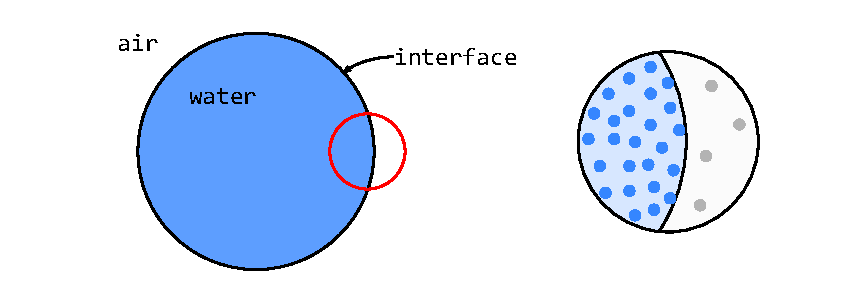
\includegraphics[width=.9\textwidth]{Pictures/moleculesAhesionCohesion_Wetting.pdf}
    \caption{Schematic of interacting molecules in a liquid droplet and its interaction with a vapor}
    \label{fig: WettingTheory_SurfaceTensionMolecules}
\end{figure}
To increase the surface area, molecules must be transported to the surface, and energy must be supplied to the system. Therefore, surface tension is also interpreted as the necessary energy required to carry a molecule to the surface.
\begin{equation}
    dE = \sigma \cdot dA
\end{equation}
with \(dE\) as the supplied energy and \(dA\) as the change in surface area.


\section{Wetting Phenomenon}
Despite the fact that the wetting of droplets is not considered in this work, it is appropriate to describe the fundamentals of wetting using this example. The concepts are the same, and many initial studies are based on this example.

In the case where the system is in equilibrium, Young \todo{ref} derived an equation relating surface tensions to the contact angle:
\begin{equation}
    \sigma_{LV} \cdot \cos\theta_e = \sigma_{SV}-\sigma_{SL}
    \label{eq: YoungsEQ}
\end{equation}
Where $\sigma_{LV}$ is the surface tension between the liquid and the gas, $\sigma_{SV}$ is from the solid to the gas, and $\sigma_{SL}$ is between the solid and the liquid (see Figure \ref{fig: YoungsLaw_ThreePhaseContactLine}).
\begin{figure}[h]
    \centering
    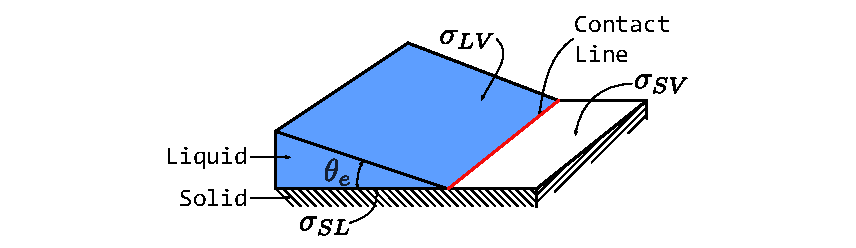
\includegraphics[width=.9\textwidth]{Pictures/YoungsLaw.pdf}
    \caption{Three Phase Contact Line}
    \label{fig: YoungsLaw_ThreePhaseContactLine}
\end{figure}
If $(\sigma_{SV}>\sigma_{SL})$ holds true, a contact angle less than $90°$ follows; otherwise, $90°\leq \theta_e<180°$. In the case where $\sigma_{SV}=\sigma_{SL}+\sigma_{LV}$, complete wetting of the surface occurs \cite{buttPhysicsChemistryInterfaces}.

When a droplet impacts a solid surface, different states can arise depending on the fluid-solid combination. At the point where the interface of the two fluids (droplet and surrounding fluid) meets the solid surface, the contact line is formed (see \ref{fig: YoungsLaw_ThreePhaseContactLine}; red line). Depending on the fluid-fluid-solid combination, a contact angle $\theta_e$ is established, where the suffix $e$ stands for equilibrium. In the case of complete wetting, the fluid spreads over the entire surface (see Figure \ref{fig: WettingTheory_WettingOfSurface} a)). This effect, however, is challenging to reproduce as it can be hindered by surface irregularities \todo{ref; i think it was butt}. As seen in Figure \ref{fig: WettingTheory_WettingOfSurface}(b-d)), states where a droplet forms on the surface are further subdivided. For a contact angle $\theta_e<90°$, it is termed hydrophilic (see \ref{fig: WettingTheory_WettingOfSurface}b)), for $\theta_e>90°$ it's hydrophobic (see \ref{fig: WettingTheory_WettingOfSurface}c)), and for a contact angle $\theta_e>120°$, it's superhydrophobic surfaces (see \ref{fig: WettingTheory_WettingOfSurface}d)). Developing superhydrophobic surfaces is also challenging.
\begin{figure}[h]
    \centering
    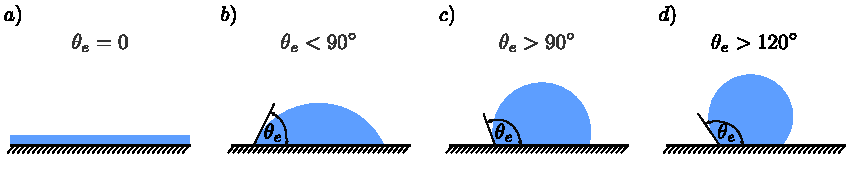
\includegraphics[width=.95\textwidth]{Pictures/DropletsAndWetting.pdf}
    \caption{Wetting of a surface}
    \label{fig: WettingTheory_WettingOfSurface}
\end{figure}
To curve the surface of the liquid, a pressure difference must exist. In the case of a sphere, Young and Laplace developed a relationship for the pressure difference in terms of the surface tension and radius as:
\begin{equation}
\label{eq: YoungLaplaceEQ}
    P_i - P_o = \Delta P =  \frac{2\sigma}{R}
\end{equation}
With $\Delta P$ being the pressure difference at the interface, $P_i$ as the pressure inside the droplet, $P_o$ the ambient pressure, and $R$ as the radius of the sphere. For a derivation, refer to \cite{buttPhysicsChemistryInterfaces}.


\subsection{Dynamic Weting}
Bisher wurden nur Zustände betrachtet, die Systeme im Gleichgewicht betrachten. Üblicherweise ist die Kontaktlinie jedoch in bewegung. Ist die Kontakilinie in Bewegung unterscheidet sich der Kontaktwinkel (dynamischer Kontaktwinkel $\theta_D$) von dem im Gleichgewichtszustand \cite{blake2006PhysicsMovingWetting}. Zur Bescheibung der Kontaktlinien dynamik wird der dynamische Kontaktwinkel, die relative geschwindigkeit der Kontatktlinie und der Gleichgewichtskontatktwinkel benötigt \cite{mohammadkarim2022ReviewPhysicsMoving, blake2006PhysicsMovingWetting, cox1986DynamicsSpreadingLiquids,huh1971HydrodynamicModelSteady,voinovHydrodynamicsWetting1977}.
Die beschreibung der Kontaktlinie ist jedoch aufgrund der tatsache schwierig, dass sich die Mikroskopische Ebene bis auf die makroskopische Ebene auswikt. 



In Abbildung \ref{fig: HDT_MKT_comp} sind verschiedene Ansichten auf die Kontatktlinie illustriert. Der rote Kreis in \textit{a)} weißt auf den betrachteten Bereich im rechts daneben stehenden bild hin und kann als eine Lupe verstanden werden. Vergrößern wir den Bereich in  \textit{a)} sieht man die interpretation der Kontatklinie aus sicht der Hydrodynamischen Theorie. Mit einem mikroskopischen Kontaktwinkel $\theta_m$ und dem dynamischen Kontaktwinkel $\theta_D$ (Abbildung \ref{fig: HDT_MKT_comp} \textit{b)}). Wird wieder auf die Kontatklinie fokussiert, sieht man die interpretation der molekular konetik Theorie (Abbildung \ref{fig: HDT_MKT_comp} \textit{c)}). Die illustrierten Punkte sollen auch hier wieder moleküle in vereinfachter Form darstellen. 



\begin{figure}[h]
    \centering
    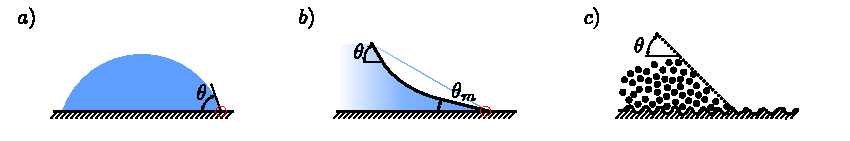
\includegraphics[width=.95\textwidth]{Pictures/ContactAngles_HDT_MKT.pdf}
    \caption{Hydrodynamic and Molecular Kinetic description of the Contact angle. Abbildung b) entsprocht dem Rot umkreisten Bereich in a), bzw. c) dem aus Bild b).}
    \label{fig: HDT_MKT_comp}
\end{figure}
\paragraph{Hydrodynamic Theory}
\label{paragraph: hydrodynTheory}
Der Hydrodynamische Ansatz löst die physik der Strömung mit Hilfe der Navier Stokes Gleichungen, bekommt jedoch bei angewandter Haftbedingung an der Kontaktlinie eine Singularität an der Kontaktlinie \cite{huh1971HydrodynamicModelSteady}. Um dieses Problem zum lösen wurde zum einen die Haftbedingung nahe der Wand gelockert oder die Lösung auf molekularer ebene beschnitten\cite{blake2006PhysicsMovingWetting}. In beiden Fällen wird eine kleine capillary number angenommen, was bedeutet, dass weit von der Kontaktlinie entfernt das Interface seine Gleichgewichtsform annimmt. 
Voinov \cite{voinovHydrodynamicsWetting1977} leitete dennoch eine Beschreibung der Kontaktlinie für einen sich ausbreitenden Tropfen in abhängigkeit der capillary number her. Eine generalisierte Variante von Cox \cite{cox1986DynamicsSpreadingLiquids} mit einigen korrekturtermen entwickelt\cite{carlsonCapillarityDynamicWetting2012,blake2006PhysicsMovingWetting}. So wird der dynamische Kontaktwinkel für $\theta_D \leq 3/4 \pi$ mit 
\begin{equation}
    \label{eq: Cox-Voinov}
    \theta_D^3-\theta_m^3= 9 Ca \ln\left(\frac{L}{L_m}\right) = 9 \frac{\mu u}{\sigma}\ln\left(\frac{L}{L_m}\right)
\end{equation}
Mit $L$ als makroskopische Weglänge und $L_m$ als mikroskopische Weglänge. Für die annahme, dass das Interface weit entfernd seine Gleichgewichtsform annimmt, wird $\theta_m = \theta_e$. Voinov selbst erkannte jedoch bereits an, dass auch $\theta_m$ anbängig von der Geschwindigkeit sein könnte\cite{voinovHydrodynamicsWetting1977,blake2006PhysicsMovingWetting}.\todo{cite lacis} 


\paragraph{Molekular Kinetic Theory}
Das Molekular Kinetik Modell beschreibt die Bewegung der Kontaktlinie mit einer statistischen Beschreibung der Molekularbewegung an der Kontaktlinie \cite{blake1969KineticsDisplacement}. 
Im gegensatz zum hydrodynamischen Modell beeinflussen die molekularen prozesse an der Kontatktlinie die der großen skalen. In dieser Betrachtung springen die Moleküle an der Kontaktlinie vor und zurück an adsorptionsstellen auf dem festen Untergrund. Die Geschwindigkeit der Kontaktlinie wird ermittelt, indem die differenz des vor und zurück springens multipliziert mit einer Sprungweite $\lambda$ multipliziert wird. Damit folgt die Beschreibung
\begin{equation}
    u=2\lambda\kappa_{0}\sinh\left(\frac{\sigma\left(\cos\theta_{e}-\cos\theta_{D}\right)}{2nk_{B}T}\right).
\end{equation}
Darin ist $n$ die Anzahl der adsorptionsstellen pro flächeneinheit, $k_0$ eine charakteristische Frequenz, $k_b$ die Boltzmann Konstante und $T$ die Temperatur.
Ist das system im Gleichgewicht, ist das vor und zurück springen im Gleichgewicht und die Kontatktlinie kommt zum stehen \cite{carlson2011DissipationRapidDynamic,blake2006PhysicsMovingWetting}. Ein Problem dieser Betrachtung ist es jedoch, dass dieses Modell eher qualitativ und rechenintensiv ist \cite{mohammadkarim2022ReviewPhysicsMoving}.







\subsection{Capillary Rise}
\label{sec: CapillaryRise}

Eine Kapillare ist ein sehr dünnes Rohr in denen durch Oberflächeneffekte eine Flüssigkeit ohne äußere Krafteinwirkung auf oder absteigt. In \ref{fig: classicCapillary} ist eine Kapillare mit bereits aufgestiegener Flüssigkeitssäule dargestellt. Darin sind ebenfall die bereits bekannten Oberflächenspannungen an ihren jeweiligen stellen markiert, sowie die wesentlichen Geometrischen parameter, wie Durchmesser ($2R$) oder höhe des entstandenen Meniskus $z$. Ebenfalls ist der resultierende Kontaktwinkel nach erreichen des Gleichgewichts gezeigt $\theta_e$. Das System in dieser Darstellung unterliegt auch Schwerkräften. 

\begin{figure}[h]
    \centering
    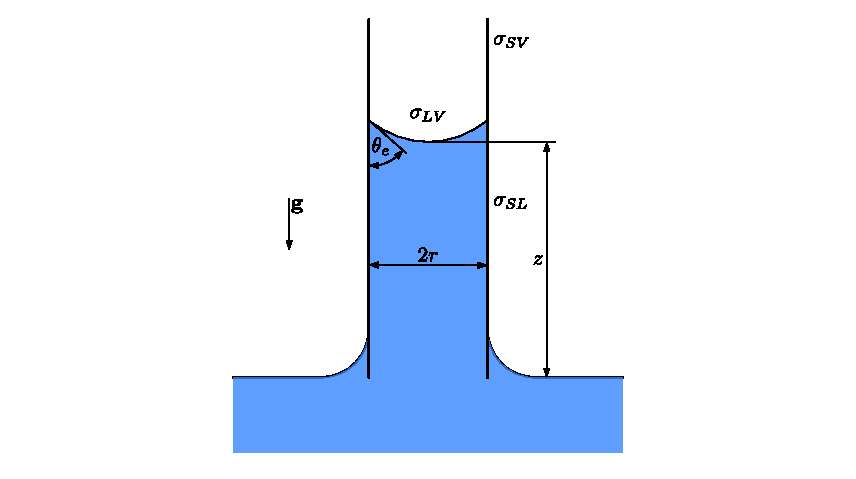
\includegraphics[width=.95\textwidth]{Pictures/classicCapillary.pdf}
    \caption{schematiche Darstellung einer Kapillare in einer Flüssigkeit nachdem diese in die Kapillare eingedrungen ist}
    \label{fig: classicCapillary}
\end{figure}
In dieser Arbeit wird ein solches System verwendet. Dabei gelten edoch weitere Bedingungen. Es wird angenommen, dass das System isobar, isotherm und die Flüssigkeit Newtonsch ist. Weiter gilt, dass während die Wassersäule in der Kapillare aufsteigt eine Poiseuille Strömung vorliegt und kein Phasenwechsel stattfindet. Weiter wird angenommen, dass die Viskosität der Gasphase vernachlässigbar ist. Mit diesen Annahmen und Randbedingungen kann die Newtondynamik in einer Kapillare als Gleichgewicht zwischen den Trägheitskräften zur Summe der Kapillaren Kräften, der Viskosen Kräfte und Hydrostatischen Kräfte \cite{fricke2023AnalyticalStudyCapillary}
\begin{equation}
\label{eq: NewtonBalanceForcesOnly}
    \frac{d}{dt}M(z,\dot{z}) = F_w - F_{\eta} - F_g
\end{equation}
Mit $M(z,\dot{z}) = \pi r^2 \rho z \dot{z}$ als das Moment, $F_g = \pi r^2 \rho g z$ als Gewichtskraft und $F_{\eta}$ als viskosen Widerstand, der sich aus der Annahme der mittleren Geschwindigkeit und vorliegenden Poiseuille Strömung zu $F_{\eta}=8\pi\eta z \dot{z}$ ergibt. Mit $\dot{z}$ als mittlere Geschwindigkeit. Die Kapillaren Kräfte folgen aus der vorherigen Beschreibung der Oberflächenspannung und der Änderung der Oberfläche des Meniskus bei änderung der aktuellen höhe zu:
\begin{equation}
    F_W=\sigma \frac{dA}{dz} = \sigma 2\pi r
\end{equation}
Die Oberflächenspannung $\sigma$ ist hierbei der zuwachs der Oberflächenenergie durch das Benetzen der festen Wand der Kapillare. Damit gilt $\sigma = \sigma_{SV}- \sigma_{SL}$. Diese Beschreibung ist bereits aus der Young Gleichung (\ref{eq: YoungsEQ}) bekannt. Damit folgt nach einsetzen für die Kapillaren Kräfte
\begin{equation}
    F_W = \sigma_{LV} \cdot \cos \theta_e 2\pi r.
\end{equation}
Damit folgt weiter für Gleichung \ref{eq: NewtonBalanceForcesOnly} nach einsetzen \cite{fricke2023AnalyticalStudyCapillary}
\begin{equation}
\label{eq: NewtonDynCapillary}
    \pi r^2 \rho \frac{d}{dt} (z \dot{z}) = \sigma_{LV} \cdot \cos \theta_e 2\pi r-8\pi\eta z \dot{z}-\pi r^2 \rho g z.
\end{equation}

Erste Beschreibungen von Bell und Cameron \cite{bell1906FlowLiquidsCapillary} haben die Aufstiegsdynamik nicht anhand von Gleichung \ref{eq: NewtonDynCapillary} beschrieben. Sie entwickelten anhand von Experimenten die Aufstiegsdynaik nach 
\begin{equation}
    z(t)^n = K\cdot t.
\end{equation}
Darin sind sowohl $n$ als auch $K$ von der Temperatur abhängige Konstanten. 1918 entwickelte Lucas \cite{lucas1918UeberZeitgesetzKapillaren} und 1921 Washburn \cite{washburn1921DynamicsCapillaryFlow} unter vernachlässigung der Trägheits- und Gravitationsterme die Lucas Washburn Gleichung wie folgt:
\begin{equation}
\label{eq: LW-Eq}
    z(t) = \sqrt{\frac{r\sigma\cos\theta_e}{2\eta}t}
\end{equation}
Damit entwickelten sie unabhängig voneinander eine Gleichung mit der der Kapillare Aufstieg anhand von Stoffwerten und Messgrößen beschrieben werden kann. Daher entwickelte sie über die Jahre große Popularität. Durch die Vernachlässigung einzelner terme und vereinafachungen im System ist diese Gleichung jedoch nicht immer präzise. Washburn selbst wies darauf hin, dass er, um die vorhersage der Gleichung zu treffen die erfolgten Experimente so aufbauen musste, dass die Kapillare prewetted wurden. 
Daher wurden für verschiedene Probleme anpassungen an diese Gleichung vorgenommen \cite{dimitrov2007CapillaryRiseNanopores, heiranian2022ModifiedLucasWashburnTheory,cai2021LucasWashburnEquationBased,fries2008AnalyticSolutionCapillary,fricke2023AnalyticalStudyCapillary,delannoy2019DualRoleViscosity,martic2002MolecularDynamicsSimulation}.Wu et al. \cite{wu2017CapillaryRiseValidity} untersuche mehrere Modelle und verglich sie mit Experimenten. 
\todo[inline]{Wu2017 \cite{wu2017CapillaryRiseValidity} untersuchte mehrere Modelle der Art, dass der dynamische Kontatkwinkel untersucht wurde. }
(\todo{cite papers; dimitrov,... check!!}. Darin wird jedoch stets angenommen, dass die Höhe des Meniskus nach $z(t)\sim \sqrt{t}$ anwächst.
Bosanquet \cite{bosanquet1923LVFlowLiquids} deutete 1923 in seiner Arbeit darauf hin, dass Gleichung \ref{eq: LW-Eq} für $t\xrightarrow{}0$ zu unphysikalischem verhalten führen wird und entwickelte ebenfalls eine Gleichung, die dieses Problem beibehielt, jedoch nun auch die Trägheit mit einbezog und für frühe Zeitpunkte der imbibition eine bessere vorhersage des Aufstiegs geben kann. \todo{cite papers. look it up you had some.}
Siegel \cite{siegel1961TransientCapillaryRise} untersuchte das Aufstiegsverhalten unter mikrogravitation und stellte ein lineares Wachstum fest. Erreichte dabei jedoch nicht das Lucas-Washburn regime. Zhmud et al. \cite{zhmud2000DynamicsCapillaryRise} wies ebenfalls auf die Probleme für Zeiten nahe $0$ aus Glecihung \ref{eq: LW-Eq} hin und beschrieb einen quadratischen zusammenhang für die zeiten, in denen das Fluid in die Kapillare gezogen wird, gefolgt von dem bekannten Lucas-Washburn Regime.
Dreyer et al. \cite{dreyer1994CapillaryRiseLiquid} untersuchte parallele Platten unter mikrogravitation und unterteile den Aufstieg des Meniskus in drei Regionen. Angefangen mit einem quadratischen Waschstum, gefolgt von einer linearen Region und abschließend dem Lucas-Washburn Wachstum. Quéré \cite{quere1997InertialCapillarity} zeigte ein lineares wachstum zu beginn indem er annahm, dass in diesem Fall nur die Trägheit eine Rolle spielt. Stange \cite{stange2003CapillaryDrivenFlow} bestätigte die drei Regionen von Dreyer et al. \cite{dreyer1994CapillaryRiseLiquid} und leitete dimensionslose Gleichungen her, um Übergangszeiten zu entwickeln. 
Fries et al. \cite{fries2008TransitionInertialViscous} teilte das Wachstumsgebiet in Bereiche ein, in denen unterschiedliche Kräfte wirken. Zu Beginn dominiert die Trägheit, gefolgt von einem übergangsgebiet in dem die viskosen kräfte übernehmen, bis sie schließlich dominieren. Auch sie entwickelten dimensionslose Zeitpunkte an denen der Übergang stattfindet. 
An dem Punkt, an dem sich die viskose Reibung und die auswirkungen von Trägheit oder dynamischen Kontaktwinkel gleichen, wurde von Quéré \cite{quere1997InertialCapillarity} und Fries et al. \cite{fries2008TransitionInertialViscous} die charakteristische Eindringlänge
\begin{equation}
    \label{eq: charLength}
    l_c \propto r \sqrt{\frac{r\rho \sigma}{\mu^2}}
\end{equation}
definiert. 



Dellanoy et al. \cite{delannoy2019DualRoleViscosity} fokusierte sich auf frühe Zeitpunkte und untersuchte viskose Fluide und bestätigte den Einfluss des prewettings der Kapillare, wie schon Washburn \cite{washburn1921DynamicsCapillaryFlow} und zeigte auch eine Abweichtung vom Lucas-Washburn regime zu frühen Zeitpunkten. Sie führten diese Abweichung auf lokale viskose dissipation in der Wedge Region zurück, statt auf eine Globale dissipation, wie sie von Lucas und Washburn angenommen wurde. Bezogen auf den dynamischen Kontaktwinkel zeigten sie, dass sich die charakteristische Eindringlänge (vgl. Gleichung \ref{eq: charLength}) nach 
\begin{equation}
    l_c \propto r \ln\left(\frac{r}{l_m}\right)
\end{equation}
berechnet. Mit $l_m$ als mikroskopische Länge, die die Singularität der Kontaktlinie ausgleicht \cite{cox1986DynamicsSpreadingLiquids}. Weiter nahmen sie an, dass sobadl $l_c$ erreicht ist, der Übergang zum Lucas-Washburn Regime erfolgt.
Ruiz-Gutiérrez et al. \cite{ruiz-gutierrez2022LongCrossoverDynamics} Wiedersprechen in ihrer Arbeit dieser aussage und zeigen, dass dieser Übergang länger verläuft. Dies Argumentieren sie damit, dass die auswirkungen von trägheit und dynamischen Kontaktwinkel nicht exponentiell abklingen. 
Dafür erweitern sie Gleichung \ref{eq: NewtonDynCapillary} für problme mit bewegendem Interface, indem sie 
\begin{equation}
    f(\dot{z}) \equiv \frac{\cos\theta_{m}-\cos\theta_D(\dot{z})}{\cos\theta_m} 
\end{equation}
einführen. Mit der Annahme, dass für $u>0$ aus Gleichung \ref{eq: Cox-Voinov} $\theta_D > \theta_m$ gilt, verschwindet diese Funktion für $\theta_D \rightarrow \theta_m$. 
Da nun das sich bewegende System betrachtet wird, wird die Gleichung \ref{eq: NewtonDynCapillary} für den in dieser Arbeit betrachteten Fall zu:

\begin{equation}
    \pi r^{2}\rho z \frac{du}{dt}= 2\pi r\sigma \cos\theta_{m}+\pi r^{2}\rho gz-8\pi \sigma z \dot{z} -2\pi r \sigma \cos \theta_{m}f
\end{equation}
Mit den ersten beiden Termen als treibende Kräfte und den letzten beiden als Widerstandskräfte. Der letzte Term ist hinzugekommen und wirkt als Korrektur für die tatsache, dass der dynamische Kontaktwinkel nicht dem makroskopischen Kontaktwinkel entspricht.

Im folgenden wurden dimensionslose größen eingeführt und vier Fälle definiert. Jeweils zwei mit großer und klener Laplace Zahl, bzw. großem und kleinen verhältnis der Längenskalen. Mit den verwendeten Größen in dieser Arbeit sollte damit der Fall drei von Ruiz-Gutiérrez et al. \cite{ruiz-gutierrez2022LongCrossoverDynamics} vorliegen. Damit sagen sie vorher, dass das Quadratische regime nicht auftreten wird und der Aufstieg mit einem linearen Gebiet beginnt und schließlich zum Lucas-Washburn Regime übergeht.






\todo[inline]{maybe use this eq instead of shorted one?}
\begin{equation}
    \pi r^2\rho l\frac{\mathrm{d}u}{\mathrm{d}t}=2\pi r\gamma\cos\theta_a+\pi r^2\rho gh-8\pi\mu lu-\frac{3}{2}\pi r^2\rho u^2-2\pi r\gamma\cos\theta_af
\end{equation}


\section{Simulating the Wetting Processes}
Die Simualation einer zwei Phasenströmung kann über mehrere Wege erfolgen. Ein üblicher weg sind die \texttt{Volume-of-Fluid} und die \texttt{Level-Set} Methode. Beide Methoden verwenden ein scharfes interface und beruhen auf der Hydrodynamischen Theorie aus Kapitel \ref{paragraph: hydrodynTheory}. Darüber hinaus sind es \textit{interface capturing} Methoden und benötigen daher keine neue neuberechnung des Rechennetzes über den Zeitraum der Simulation. Andere Methoden, die dem Interface folgen (\textit{interface tracking}), sind auch möglich. Einer der größten nachteile der genannten Methoden ist es, dass die bewegte Kontatktlinie bei verwendung der Haftbedingung von Modellen abhängig ist\cite{carlsonCapillarityDynamicWetting2012}. Darüber hinaus kann die Berechnung der Oberflächenspnnung ein Problem darstellen. Hier muss die Krümmung der Oberfläche berechnet werden, was zu vergleichsweise hohen numerischen Fehlern führen kann \cite{jamshidi2019SuitabilityPhasefieldAlgebraic,hagg2019DirekteNumerischeSimulation}. 
Die Lattice-Boltzmann Methode verwendet Kollisionsmodelle, um das Verhalten des Fluids zu beschrieben. Grenzflächenspannungen können durch Modifikationen berücksichtigt werden. Hier gibt es ansätze, die vielversprechend sind und einige auch mit der Phasenfeld Methode vergleichbar sind. Jedoch ist eins der größten Probleme die limitierung der Dichte oder Viskositätsverhältnisse. In dieser Arbeit haben die Fluide stark unterschiedliche Dichten mit einem Verhältnis von $1000$. Die Lattice-Boltzmann Methode ist jedoch nach \cite{chenCriticalReviewPseudopotential2014} für Verhältnisse von $\mathcal{O}(10)$ limitiert und führt ansonsten zu instabilitäten. 
Ein weitere häufig verwendete Methode sind \texttt{Molecular Dynamic} Simulationen. Da in diesem Fall Moleküle einzeln Simuliert werden, ist diese Methode nur auf Geometrisch und zeitlich kleine Probleme anwendbar, ohne die Computational costs zu hoch zu treiben. Daher werden {Molecular Dynamic} Simulationen oft zum Vergleich herangezogen, oder um nur kleine Probleme zu betrachten (\cite{datta2023EarlyStageLiquidInfiltration,lacisNanoscaleShearedDroplet2022,martic2002MolecularDynamicsSimulation,dimitrov2007CapillaryRiseNanopores})
Die in dieser Arbeit verwendete Methode ist die Phasenfeld Methode. Diese metohde modelliert die zwei oder auch mehrphasenströmung über die freie Energie des Systems. Eine genauere Beschreibung dieser Methode und bereits durcgeführten Simulationen erfolgt in Kapitel \ref{chap: PhaseFieldMethod}. \todo[inline]{Elaborate or maybe move entire section to phase field? Or maybe case setup with a reasoning why phasefield? }
